\documentclass[../Notes_of_CaRiVaC.tex]{subfiles}

\begin{document}
\chapter{Spatial And-Or Graph}%
\label{sec:ii.2}
The proposal grammar integrates three representations:
%
\begin{enumerate}
  \item Stochastic grammars for composition.
  \item Markov (or graphical) models for contexts.
  \item Sparse coding with primitives (wavelets).
\end{enumerate}
%

\section{Three New Issues in Image Grammars in Contrast to Language}%
\label{sec:ii.2.1}
An image grammar should include two aspects:
%
\begin{enumerate}
  \item The hierarchical structures $\mathcal{G}$ which generate a set of valid
    image configurations $\mathbf{L}(\mathcal{G})$.
  \item The context information which makes sure the components in a
    configuration observe good spatial relationships between object parts,
    e.g.\ relative positions, ratio of sizes, consistency of colors.
\end{enumerate}
%

There are three major differences (and difficulties) between the language
grammars and image grammars.

\textbf{First, the loss of the left-to-right ordering in language.} In
language, every production rule $A \to \beta$ is assumed to generate a linearly
ordered sequence of nodes $\beta$ and following this down to the leaves, we get
a linearly ordered sequences of terminal words. In vision, we have to replace
the implicit links of words to their left and right neighbors by the edges of a
more complex ``region adjacency graph'' (RAG). That is, let an image $I$ have a
decomposition $D = \cup_{k \in S} R_k$, where a RAG is made with nodes
$\langle R_i \rangle$ and edges are represented as
$\langle R_k \rangle \text{\textemdash} \langle R_l \rangle$ whenever adjacent,
then the nodes of $\beta$ in $A \to \beta$ are no longer linearly ordered.
Instead, $\beta$ should be made into a configuration which is a set of nodes
from $V_N \cup V_T$ plus horizontal edges representing adjacency.

\newpage

\begin{textbox}{\textit{Original Texts}}
One immediate consequence of the lack of natural ordering is that a region has
very ambiguous production rules. Let $A$ be a region and $a$ an atomic region,
and let the production rule be $A \to aA \vert a$. A linear region
$\omega = (a, a, a, \ldots, a)$ has a unique parse graph in left-to-right
ordering. With the order removed, it has a combinatorial number of parse trees.
\Fig{ii.2.1} shows an example of parsing an image with a cheetah. It becomes
infeasible to estimate the probability $p(\omega)$ by summing over all these
parse trees in a grammar.
\end{textbox}
%
\begin{figure}[!htpb]
  \centering
  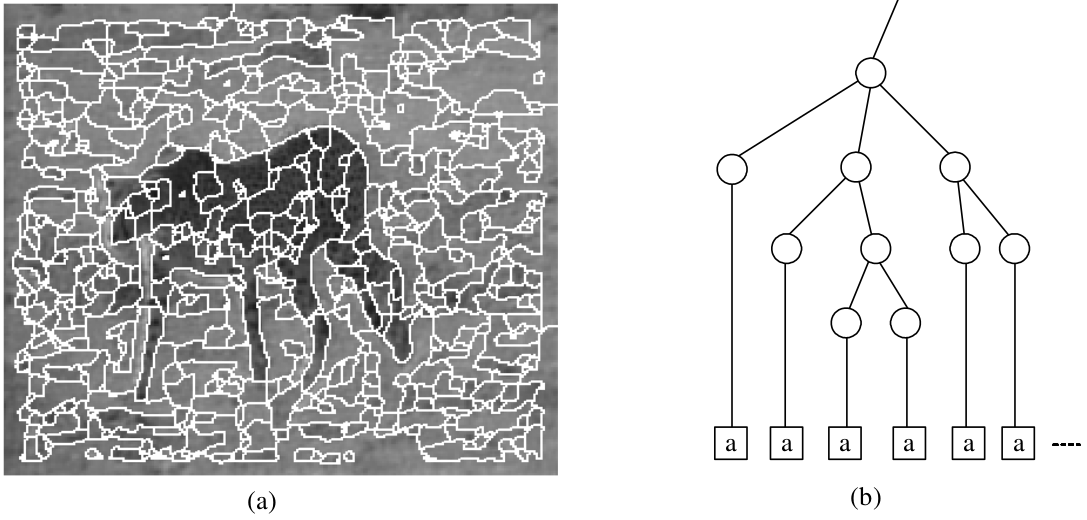
\includegraphics[width=0.65\linewidth]{fig_ii_2_1.png}
  \caption{A cheetah and the background after local segmentation: both can be
    described by a RAG\@. Without the left-to-right order, if the regions are
    to be merged one at a time, they have a combinatorially explosive number
of parse trees.}%
  \label{fig:ii.2.1}
\end{figure}
%

Therefore we must avoid recursively define $A \to aA$, and treat the grouping
of atomic regions into one large region $A$ as a \textbf{single computational
step}, such as the grouping and partitioning in a graph space\cite{barbu2005}.
\textbf{Thus $p(\omega)$ is assigned to each object as a whole instead of the
production rules.}

%
\begin{figure}[!htpb]
  \centering
  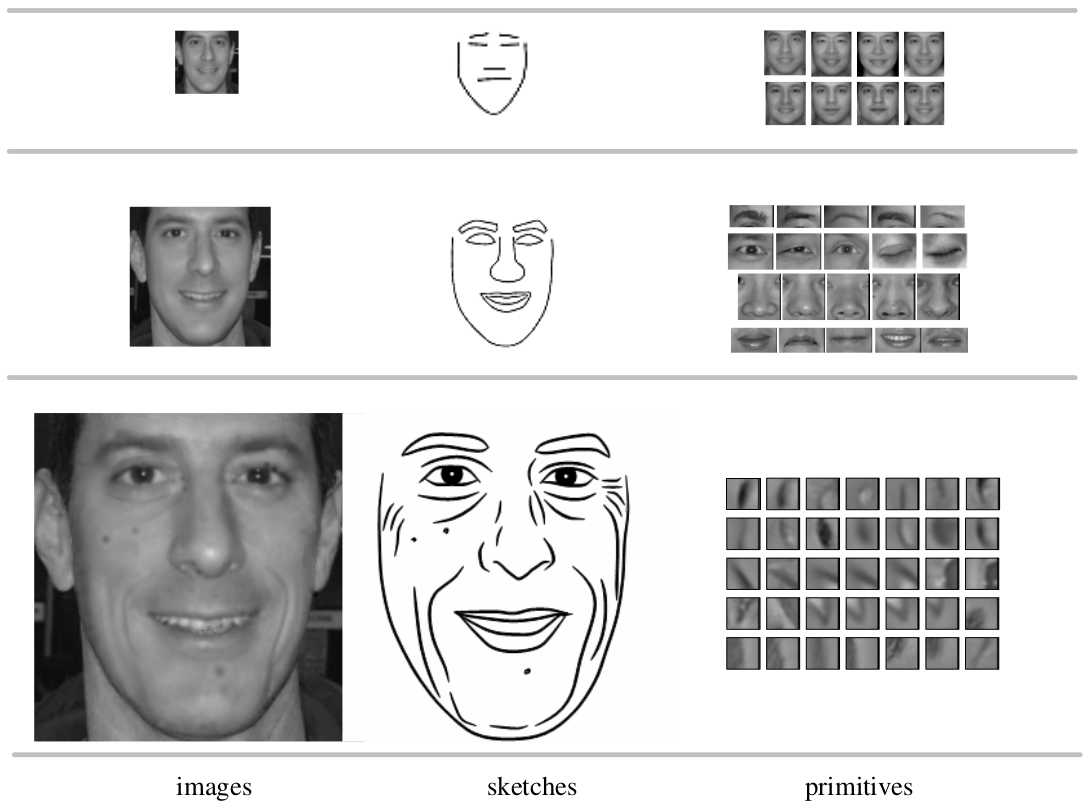
\includegraphics[width=0.6\linewidth]{fig_ii_2_2.png}
  \caption{A face appears at three resolutions is represented by graph
    configurations in three scales. The right column shows the primitives used
  at the three levels.}%
  \label{fig:ii.2.2}
\end{figure}
%

\textbf{Second, the issue of scaling is unseen in language grammar.} This
implies that the parse tree can terminate immediately at any node because no
more details is visible.

\Fig{ii.2.2} shows an example of such issue. One can add some termination rules
to each non-terminal node, e.g., each non-terminal node may exit the production
for a low resolution case:
%
\begin{align}
  \label{eq:ii.2.1}
  \forall A \in V_N, A \to \beta_1 \vert \cdots \vert \beta_{n(A)} \vert t_1 \vert t_2
\end{align}
%
where $t_1, t_2 \in V_T$ are image primitives or image templates for $A$ at
certain scales. This issue does not complicate the grammar design, except that
one must learn the image primitives at multiple scales in developing the visual
vocabulary.

\textbf{Third, natural images contain a much wider spectrum of quite irregular
local patterns than in speech signals.} Images have: (i) very regular and
highly structured objects which could be composed by \textbf{production rules};
(ii) very stochastic patterns such as clutter and texture which are better
represented by \textbf{Markov Random Field (MRF)} models. The spectrum is
continuous {\color{red} (?)}. The structured and textured patterns can transfer
from one to the other through continuous scaling\cite{wang2008}\cite{wu2008}.

\section{Visual Vocabulary}%
\label{sec:ii.2.2}
\subsection{The Hierarchical Visual Vocabulary \textendash~the ``Lego Land''}%
\label{sec:ii.2.2.1}
\begin{textbox}{\textit{Definition I. Visual Vocabulary}}
The visual vocabulary is a set of pairs, each consisting of an image function
$\Phi_i(x, y; \alpha_i)$ and a set of $d(i)$ bonds (i.e., its degree), to be
eventually connected to with other elements, which are denoted by a vector
$\beta_i = (\beta_{i,1}, \ldots, \beta_{i, d(i)})$. We think of $\beta_{i,k}$
as an \textbf{address variable or pointer}. $\alpha_i$ is a \textbf{vector of
attributes} for (a) a geometric transformation, e.g.\ the central position,
scale, orientation and plastic deformation, and (b) appearances, such as
intensity contrast, profile or surface albedo. In particular, $\alpha_i$
determines a domain $\Lambda_i(\alpha_i)$ and $\Phi_i$ is then defined for
$(x, y) \in \Lambda_i$ with values in $R$ (a gray-valued template) or $R^3$ (a
color template). Often each $\beta_{i,k}$ is associated with a subset of the
boundary of $\Lambda_i(\alpha_i)$. The whole vocabulary is thus a set:
%
\begin{align}
  \label{eq:ii.2.2}
  \Delta = \{(\Phi_i(x, y; \alpha_i), \beta_i): (x, y) \in  \Lambda_i(\alpha_i) \subset \Lambda\}
\end{align}
%
where $i$ indexes the type of the primitives.
\end{textbox}

The conventional wavelets, Gabor image bases, image patches, and image
fragments are possible examples of this vocabulary except that they don't have
bonds.

\subsection{Image Primitives}%
\label{sec:ii.2.2.2}
Julesz conjectured that textons are the atomic elements in the early stage of
visual perception for local structures. Marr extended texton concept to image
primitives which called ``symbolic tokens'' --- primal sketch.

As illustrated in \Fig{ii.2.3}\.(a), an image primitive is a small image patch
with a degree $d$ connections or bonds illustrated by the half circles:
%
\begin{itemize}
  \item blobs ($d$ = 0)
  \item terminators ($d$ = 1)
  \item edges/ridges ($d$ = 2)
  \item ``L''-junctions ($d$ = 2)
  \item ``T''-junctions ($d$ = 3)
  \item cross junctions ($d$ = 4)
\end{itemize}
%
\begin{figure}[!htpb]
  \centering
  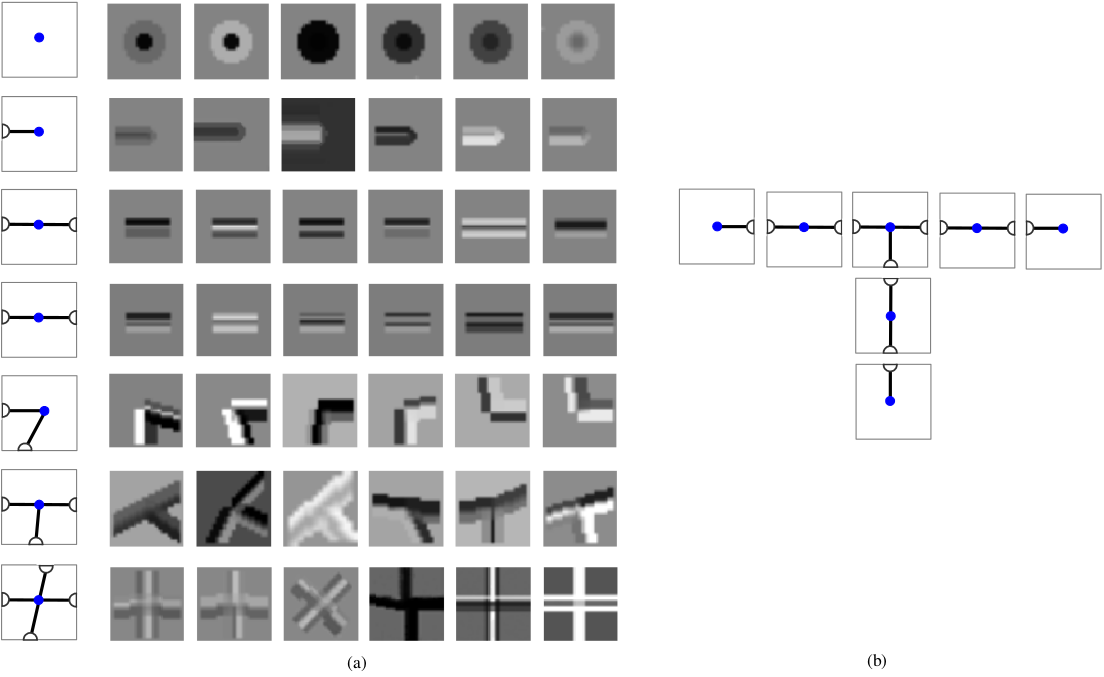
\includegraphics[width=0.8\linewidth]{fig_ii_2_3.png}
  \caption{Low level visual vocabulary \- image primitives. (a). Some examples
    of image primitives: blobs, terminators, edges, ridges, ``L''-junctions,
    ``T''-junction, and cross junction etc. These primitives are the elements
    for composing a bigger graph structure at the upper level of the hierarchy.
    (b) is an example of composing a big ``T''-shape image using 7 primitives.
    From (Guo, Zhu and Wu, 2003).}%
  \label{fig:ii.2.3}
\end{figure}
%


\end{document}
